

\section{Introduction}

\subsection{Motivation}

\indent The exponential growth of client-server distributed applications has led to a need for them to be scalable systems able to service many users. Many applications currently rely on static configurations or topologies, which could limit their ability to change scale and adapt to changes in traffic. This inflexibility potential could cause increased latency and even service outages. This is because static topology configurations can perform well overall depending on the situation; however; for the internet, there is not a one size fits all solution, and a simple switch of topology to compensate for weaknesses of the previous could lead to a tremendous performance and robustness increase. For example, popular client-server distributed applications like Zoom struggled during the early COVID-19 pandemic because their current infrastructure limited their scalability, fault-tolerance, and efficiency during the surge of the increased nodes and geographical distribution of nodes. Ultimately, this problem that plagued the video calling platforms was fixed using edge computing and CDNs; however, changing topologies could have also increased the distributed system's scalability.

This leads to the question: How does switching the topology in a distributed client-server setting affect the performance and, therefore, the scalability of the distributed application? Therefore, the vision for this study is to lead the way for revolutionizing the scalability and performance of client-server distributed applications by conducting simulations to see if there is a positive relationship between changing the topology and performance of the distributed system. It is imperative to address this problem to ensure the continued growth of client-server distributed applications to maintain user satisfaction.

Thus the novelty of our study comes from the approach to changing the topologies in a distributed setting to find out if there is a relationship between the performance of a distributed application and changing the topology. Other solutions to increase scalability and preformance that have appeared, like CDNs and edge computing, do not relate to changing topology. 

The key results of this study show that changing the topology could lead to performance benefits for some distributed applications with the small caveat that one could benefit while others could not or in fact, decrease in performance. This opens up the way for developing solutions to dynamically manage the topology's structure to leverage those performance boosts. Therefore, increasing the performance and scalability of future applications. In addition, the implications of this study could be the increased use of client-server technology in distributed applications, as businesses may be interested in its increased performance and reliability. It could also contribute to the understanding and previously unknown insights into client-server networks. Lastly, It could be of value to researchers working on related topics leading to even more innovation in the future. In addition, Future work could be done to leverage the advantages to make a solution to manage the topology to enhance the scalability and performance of an application.




\subsection{Methods of Changing Topologies}

\indent Currently, as this study defines it \cite{hall_survey_2021}, the main methods of topology reconfiguration is using an Optical Transport Network (OTN) and routing protocols. The study says that the two primary methods of changing a server topology are Software-Defined Networking (SDN) and optical switches, which can change these fiber connections. SDNs, as defined by \cite{kurose2021computer}, are part of the network stack that decides the routing for packets for each router which, therefore, can change the network's topology by simply changing the routes for packets. OTN is a protocol that allows optical networks a reliable and efficient way of transporting data across a network. Furthermore, optical switches can change the topology by directly switching one optical signal to another. These are widely used in data centers, and more helpful information can be found at \cite{nandi2022optical}. Thus, this study will explore the switching of topologies under these methods.



\section{Related Work}
%\blindtext

There has been exploration already into how optical switches affect data centers preformance done by \cite{xue2023optical}. They define metrics for a datacenters preformance, such as scalability, flexibility, and efficiency, and introduce currently used topologies, fat-trees. The authors claim that optical switches will be the solution for scalability, listing out different types of switches and their speeds. This study claims that optical switches will increase scalability; however, it must demonstrate how effective enough for readers to be convinced. Therefore, our study aims to do more than the one previously described by actually conducting experiments to support the claims made by this paper.

	In addition, an existing solution already explores dynamically changing topology \cite{wen2018dynamic} for distribution systems. The solution proposed by the authors is a step in the right direction for dynamic reconfiguration for a distributed application. Although, it only considers changing topology upon nodes joining and leaving the network. Also, the authors need to evaluate their solution to a benchmark making the data they attained non-comparable or rightfully interpretable, leading their claims to be mere speculation. Therefore, before diving into a potential solution, it's essential to investigate which topology changes can enhance the system, and this is what our study aims to do, which is to explore what these beneficial changes are before actually making a dynamic topology switcher.

Existing solutions that explore testing different topologies, such as \cite{singla2012jellyfish}, explore working with a random-graph topology instead of a fat-tree topology to support more data center server nodes. They claim that using a random graph instead of a traditionally used fat-tree topology increases capacity by 25\%. The authors show that their solution outperforms others in scalability and performance. Also, showing that their random graphs topology scheme could outperform fat trees. However, it only compares one topology to another in a data center setting. It needs to tackle the problem that this study is trying to solve, which is to see how switching a topology could affect distributed applications. Therefore, it does not make claims for the casual relationship that this study aims to find between changing the topology and performance of the distributed system

%\Blindtext

\section{System Design}

\subsection{Approach}

To test if changing the topology affects the performance of a distributed system, we will test multiple topologies with different client-server setups and then change the topology and compare the performance metrics between them. To accomplish this goal, we will simulate a distributed system on top of an actual topology from The Internet Topology Zoo called AGIS. For the distributed system that is being simulated, we are using the benchmark TPC-H made by the Transaction Process Preformance Council (TPC).

	We use the AGIS topology for the simulation to reflect a real-world client-server system. Therefore, for transmitting data across the network, we only consider propagation delay calculated using the haversine distance between the coordinates of each edge of the graph.

The TPC-H benchmark comes with a database generator with business-related queries and data modifications that simulate distributed systems involving data warehousing, business intelligence, decision support systems, and online analytical processing. Therefore, the reason for including TPC-H is to simulate these groups of distributed systems in a distributed environment closely related to those in the real world.

	The challenges of this study came from inexperience in doing research and unfamiliarity with simulation frameworks like OMNet++. However, with a lot of time and guidance, we were able to make a competent simulation and complete this study.

	Our proceeding simulations occur in OMNeT++ using an SQLite version of the TPC-H database converted by \cite{lovasoaTPCHsqlite}, and queries are manually tweaked to fit with SQLite. The server nodes that host the database sessions are also presumed to be single-threaded in these scenarios. For the hardware, we are working with an Ubuntu virtual environment with 3 CPU’s and only one is given to the OMNet++ simulator. All the source code for the simulations performed, the queries, and the ned files are all original creations by this study and can be found at \cite{alex21topology}.



\subsection{Simulation Setup and Relevant Metrics}

	The simulations will consist of at least one single-threaded server and one client sending queries to the server to satisfy. For these simulations, we only assume propagation delay calculated using haversine coordinates and the speed of light through fiber optics. Additionally, the servers will host SQLite database sessions to satisfy client queries. Each client also has a set of 22 queries to send to the server.

	The simulations performed in this study consist of a one server, one client scenario, a one server multi-client scenario, and a multi-server multi-client scenario. Each will have an original and changed topology, with performance metrics for each that we will compare and contrast.

The relevant metrics from TPC-H that will be used are throughput tests and queries per hour. The throughput test measure how fast multiple streams of queries can be executed, so a client with 22 queries would be considered a stream. The metric the throughput tests provide is helpful to what clients complete their streams before others, so we can reason why that is, and we can compare the performance of the original and new topologies. Lastly, the quries per hour metric was collected to convey how efficiently the distributed system performs over time. It works by running our simulation for an hour and then multiplying the number of queries the server satisfies by the scale factor of 0.01. We set it so low because our weak hardware would make any query take seconds on end and was unsuitable for this kind of simulation. This measurement is helpful in our study because we can compare the queries per hour with our original topology to another to conclude if there are any performance benefits.




\begin{figure}[tp]
\centering
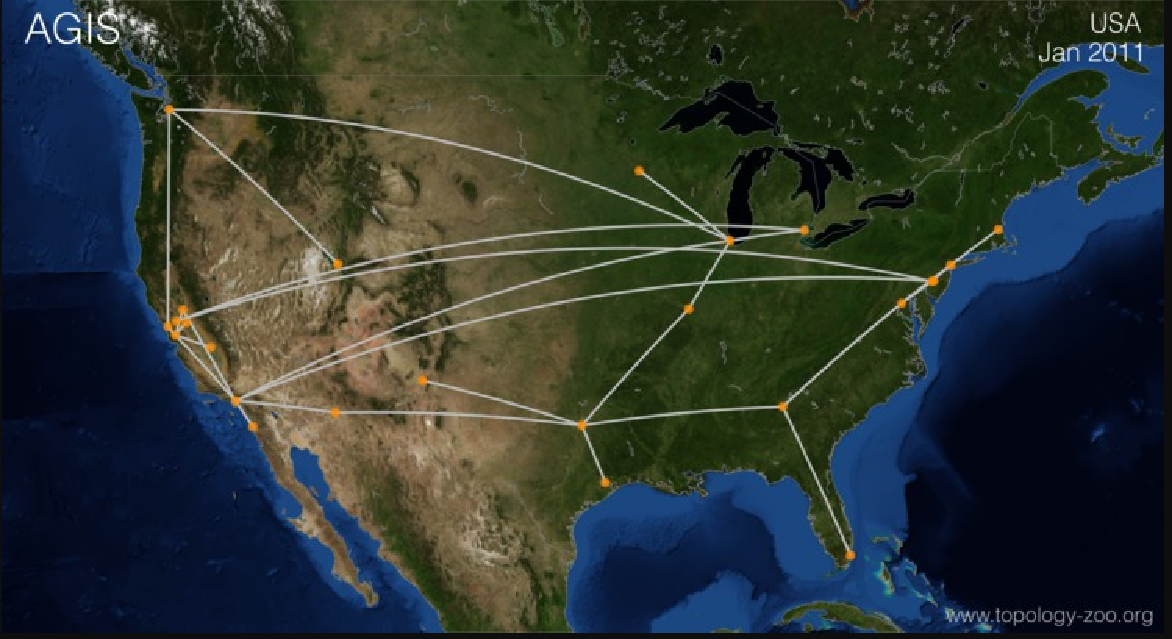
\includegraphics[width=0.5 \textwidth]{figures/AGIS_ORIG}
\caption{This is a picture containing the original AGIS topology.
}
\end{figure}

\section{Simulations}

\subsection{One Server One Client Scenario}

\begin{figure}[tp]
\centering
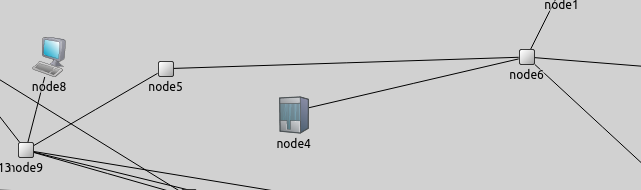
\includegraphics[width=0.5 \textwidth]{figures/SingleClientOrig}
\caption{This is the one server multi-client original topology where the clients are denoted as computers, and the server is shown as a server. Client node 8 is located at the top left and the server node 4 is shown to be in the middle.
}
\end{figure}

\begin{figure}[tp]
\centering
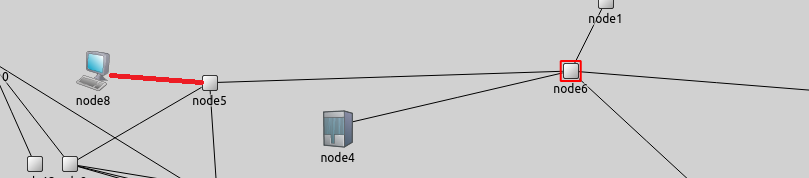
\includegraphics[width=0.5 \textwidth]{figures/SingleClientNew}
\caption{This is the one server multi-client new topology where the clients are denoted as computers, and the server is shown as a server. Client node 8 is located at the top left, and the server node 4 is shown to be in the middle. Notably, the topology changed by removing the client's only connection and replacing it with a connection to node 5, reflected in red above.
}
\end{figure}

\begin{table}[h!]
\centering
\begin{tabular}{|c|c|c|}
\hline
Server Node & Old Topology QPH & New Topology QPH \\ \hline
Server 4 & 247.2 & 249 \\ \hline
\end{tabular}
\caption{Queries per hour at scale factor 0.01 for Server node 4 under old and new topologies in the one server one client scenario.}
\label{tab:my_label}
\end{table}


\begin{table}[h!]
\centering
\begin{tabular}{|c|c|c|}
\hline
Topology & Average Time (Seconds) \\ \hline
Old & 3.15 \\ \hline
New & 3.07 \\ \hline
\end{tabular}
\caption{Average time to for the server to service the client under old and new topologies in the one server one client scenario.
}
\label{tab:avg_time_all_clients}
\end{table}


For the one server, one client scenario, we randomly assigned the server and client node to a random node in the system, creating our original topology, as shown in fig 2. We then extract performance metrics from the original topology for the throughput and queries per hour tests. We first conducted 10 throughput tests, which yielded an average time of 3.15s for the server to process all of the client's queries, as seen in Table 2. Then we conducted 10 simulations to record the queries per hour, which, with a scale factor of 0.01 on the database size, yielded an average queries per hour of 247.2 on the original topology, as seen in Table 1.

	With the baseline metrics now set by the original topology, we need to see if we can change the topology to yield better metrics than our baseline. Therefore, we can reduce the latency between the client and server nodes by making the path between them shorter. Thus, by changing the client's connection to node 5, as seen in Fig 3, we will call this our new topology, rerun our simulations, and extract performance metrics for our new topology.

	We conduct the same simulations with the new topology and extract the same metrics as we did with the original topology. The 10 throughput tests yielded an average completion time of 3.07s, as seen in Table 2. The completion times of each client node in the throughput test are shown in Table 5. Lastly, we did 10 queries per hour tests on the new topology and got an average of 249, as seen in Table 1.


\subsection{One Server One Client Results and Discussion}

	Comparing and contrasting the old topology to the new one, we can see that the new one performed slightly better based on the metrics. Specifically, with the new topology, the server can perform slightly more queries per hour and complete a set of queries from the client slightly faster. This provides sufficient evidence to claim that in a one client-server distributed application, decreasing the latency between the client and server nodes by changing the topology increased the efficiency of the distributed system. In addition, by increasing the system's efficiency, we also increase scalability.



\subsection{One Server Multi-Client Scenario}

\begin{figure}[tp]
\centering
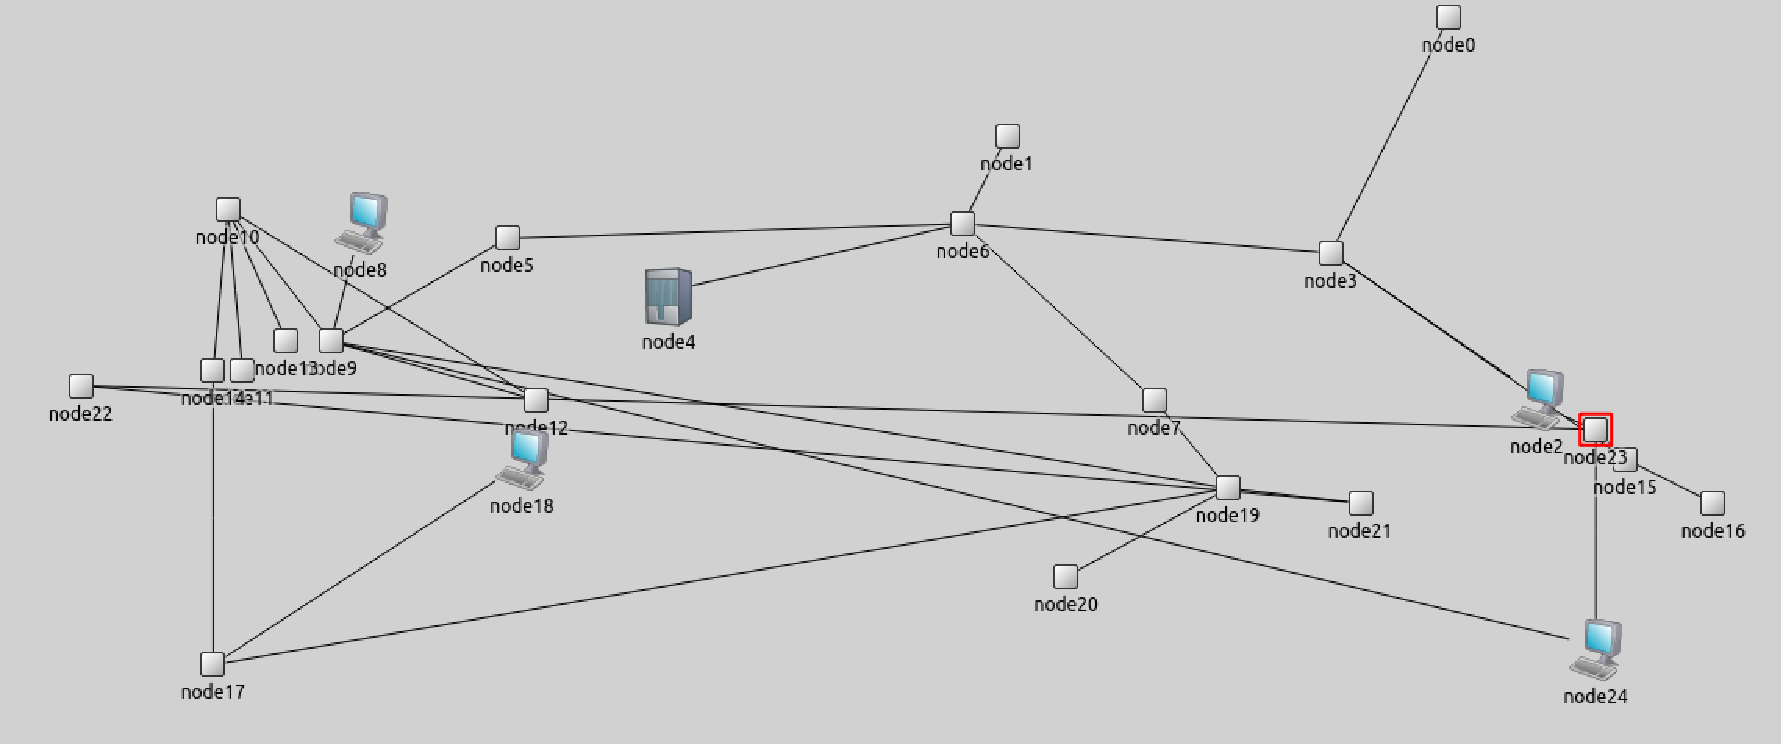
\includegraphics[width=0.5 \textwidth]{figures/MultClientOrig}
\caption{This is the one server multi-client original topology where the clients are denoted as computers, and the server is shown as a server. Client node 8 is located at the top left, client node 18 is at the bottom right, client node 2 is in the middle right, and client node 24 is at the bottom right.
}
\end{figure}

\begin{figure}[tp]
\centering
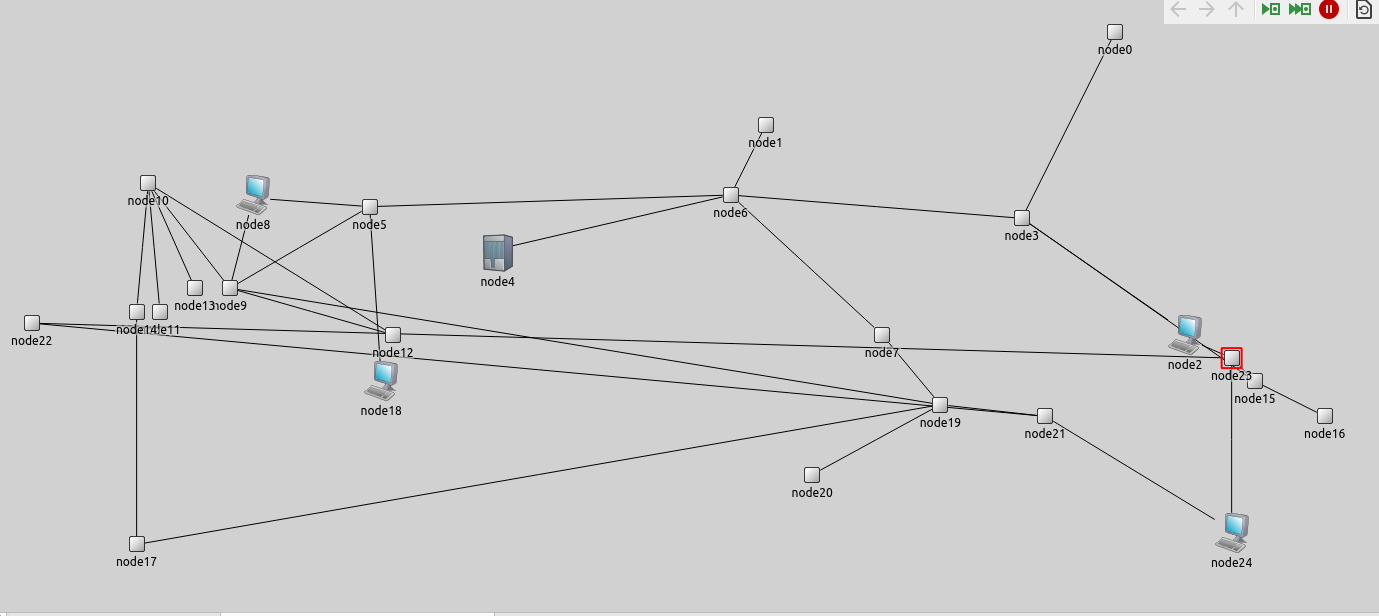
\includegraphics[width=0.5 \textwidth]{figures/MultClientNew}
\caption{This is the one server multi-client new topology where the clients are denoted as computers, and the server is shown as a server. Client node 8 is located at the top left, client node 18 is at the bottom right, client node 2 is in the middle right, and client node 24 is at the bottom right. The changes are that node 18 has a path to node 5, client node 8 connects to node 5, and lastly, client node 24 has a connection to node 21. All the changes can be seen in red.}
\end{figure}

\begin{table}[h!]
\centering
\begin{tabular}{|c|c|c|}
\hline
Server Node & Old Topology QPH & New Topology QPH \\ \hline
Server 4 & 318.6 & 333 \\ \hline
\end{tabular}
\caption{Queries per hour based on all clients at a scale factor of 0.01 for Server node 4 under old and new topologies in the one server multi-client scenario.}
\label{tab:my_label}
\end{table}


\begin{table}[h!]
\centering
\begin{tabular}{|c|c|c|}
\hline
Server Node & Old Topology (s) & New Topology (s) \\ \hline
Server 4 & 10.39 & 9.91  \\ \hline
\end{tabular}
\caption{Average time to service all clients for Server node 4 under old and new topologies in the one server multi-client scenario.}
\label{tab:average_time}
\end{table}

\begin{table}[h!]
\centering
\begin{tabular}{|c|c|c|}
\hline
Client Node & Old Topology (s) & New Topology (s) \\ \hline
Node 2 & 7.74 & 9.22  \\ \hline
Node 8 & 8.52 & 9.47 \\ \hline
Node 18 & 10.39 & 9.91 \\ \hline
Node 24 & 8.72 & 9.76 \\ \hline
\end{tabular}
\caption{Average time for each client node to complete its set of queries under old and new topologies in the one server multi-client scenario.}
\label{tab:avg_time_per_node}
\end{table}


For the one server multi-client scenario, we consider a 4-client 1-server scenario; the additional nodes are randomly assigned a geographic location, as shown in Fig 4, for which we will consider the original topology. For this topology, we simulated to extract metrics for the throughput test and queries per hour. We first conducted 10 throughput tests, which yielded an average time of 10.39s for the server to process all of the client's queries, as seen in Table 4.  Also, notably, all the client's completion times for the throughput test are in Table 5. Then we conducted 10 simulations to record the queries per hour, which, with a scale factor of 0.01 on the database size, yielded an average queries per hour of 318.6 on the original topology, as seen in Table 6.
	
	Table 5 shows that node 2, node 8, and node 24 are relatively complete around the same time, while node 18 lags a noticeably large margin behind the other client nodes. Noticeably the client nodes with a closer travel distance to the server node have lower completion times. This is because, in this simulation, the server is single-threaded meaning it can only serve one client at a time, so the clients that are first to get in line will be serviced before others leading to them completing their set of queries faster than others. For example, client node 18 is the slowest to complete its queries because messages must travel inefficiently, going away from the server, as seen in Fig 4. Using this information, we can try to improve node 18’s performance by repeating what we did with the last scenario making node 18’s path shorter to the server node. Therefore, as seen in Fig 5, we can add a connection from node 18 to node 5 for the new topology, decreasing its travel distance.

	In addition, the other client nodes could lower their latency with the server by adding connections to make the routes more efficient. For example, client node 8 could connect to node 5, like in the one server scenario. Then, client node 24 could change its connection to node 21, potentially lowering its message travel times. These changes make up the new topology in Fig 5, which can be seen in red.

	With the changes performed, we conduct the same simulations and extract the same metrics as we did with the original topology. The 10 throughput tests yielded an average completion time of 8.01s, as seen in Table 4. The completion times of each client node in the throughput test are shown in Table 5. Lastly, 10 queries per hour tests on the new topology yielded an average of 333, as seen in Table 3.



\subsection{One Server Multi-Client Results and Discussion}

	Comparing the two topologies' performances, the queries per hour and throughput tests were noticeably better for the new topology. Specifically, the old topology averaged 318.6 queries per hour, while the new topology averaged 333, which is a slight improvement overall. Therefore, this simulation provides evidence that the server's queries per hour increase when the latency between the clients and server is decreased by making a shorter path for the client nodes to the server node. Continuing, for the average completion time for the server to complete all client node queries extracted by the throughput tests, the new topology performed around half a second faster than the old topology seen in Table 4. Therefore, for a multi-client setting, shorter paths between the client and server nodes lead to the server satisfying all client node queries faster. These both, in turn, benefit the performance of the distributed system overall hence showing that changing the topology can have a positive impact on a distributed system.

Another thing to notice is that in Table 5, the completion times of the client nodes in the new topology are all around the same time as opposed to the old topology, which has more scattered times. The convergence of times for the clients in the new topology is because since some of the client nodes' latency decreased due to the topology change, all client nodes have a reasonable chance to be first in line to get query the server. That is why the previously closest nodes increased in completion time in the new topology.


\subsection{Multi-Server Multi-Client Scenario}

\begin{figure}[tp]
\centering
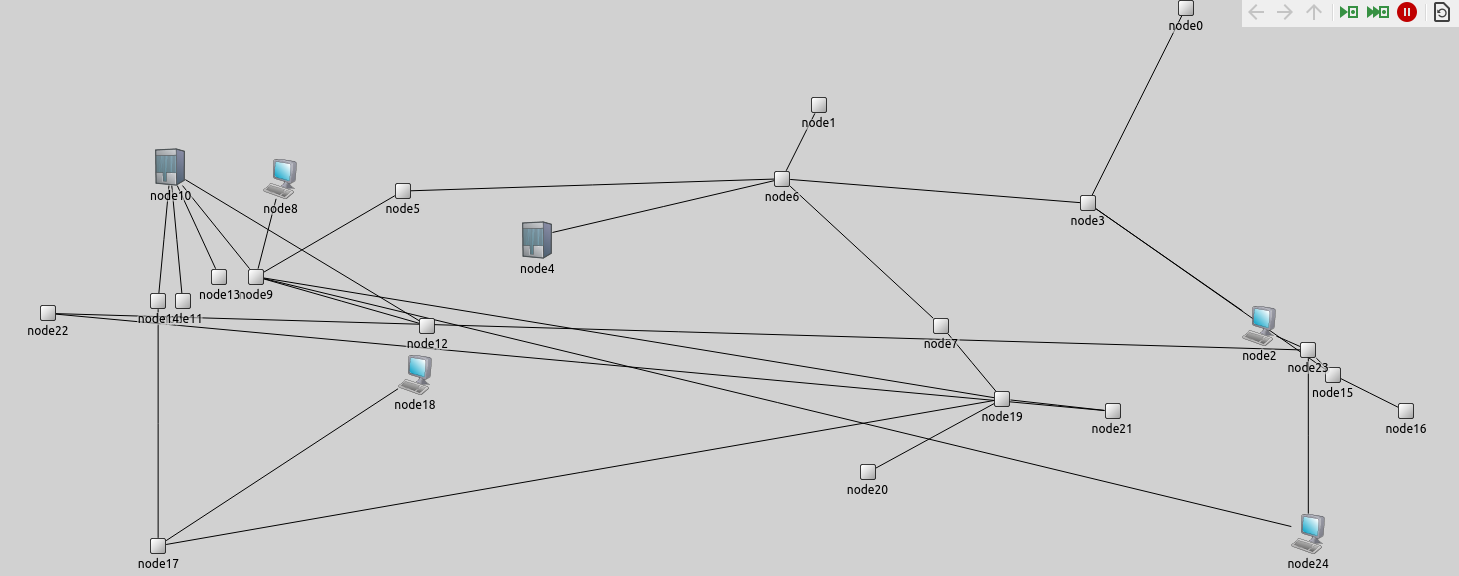
\includegraphics[width=0.5 \textwidth]{figures/MultServerOrig}
\caption{This is the multi-server multi-client original topology where the clients are denoted as computers, and the servers are shown as servers. Client node 8 is located at the top left, client node 18 is at the bottom right, client node 2 is in the middle right, and client node 24 is at the bottom right. Then server node 4 is in the middle, and server node 10 is in the upper left.
}
\end{figure}

\begin{figure}[tp]
\centering
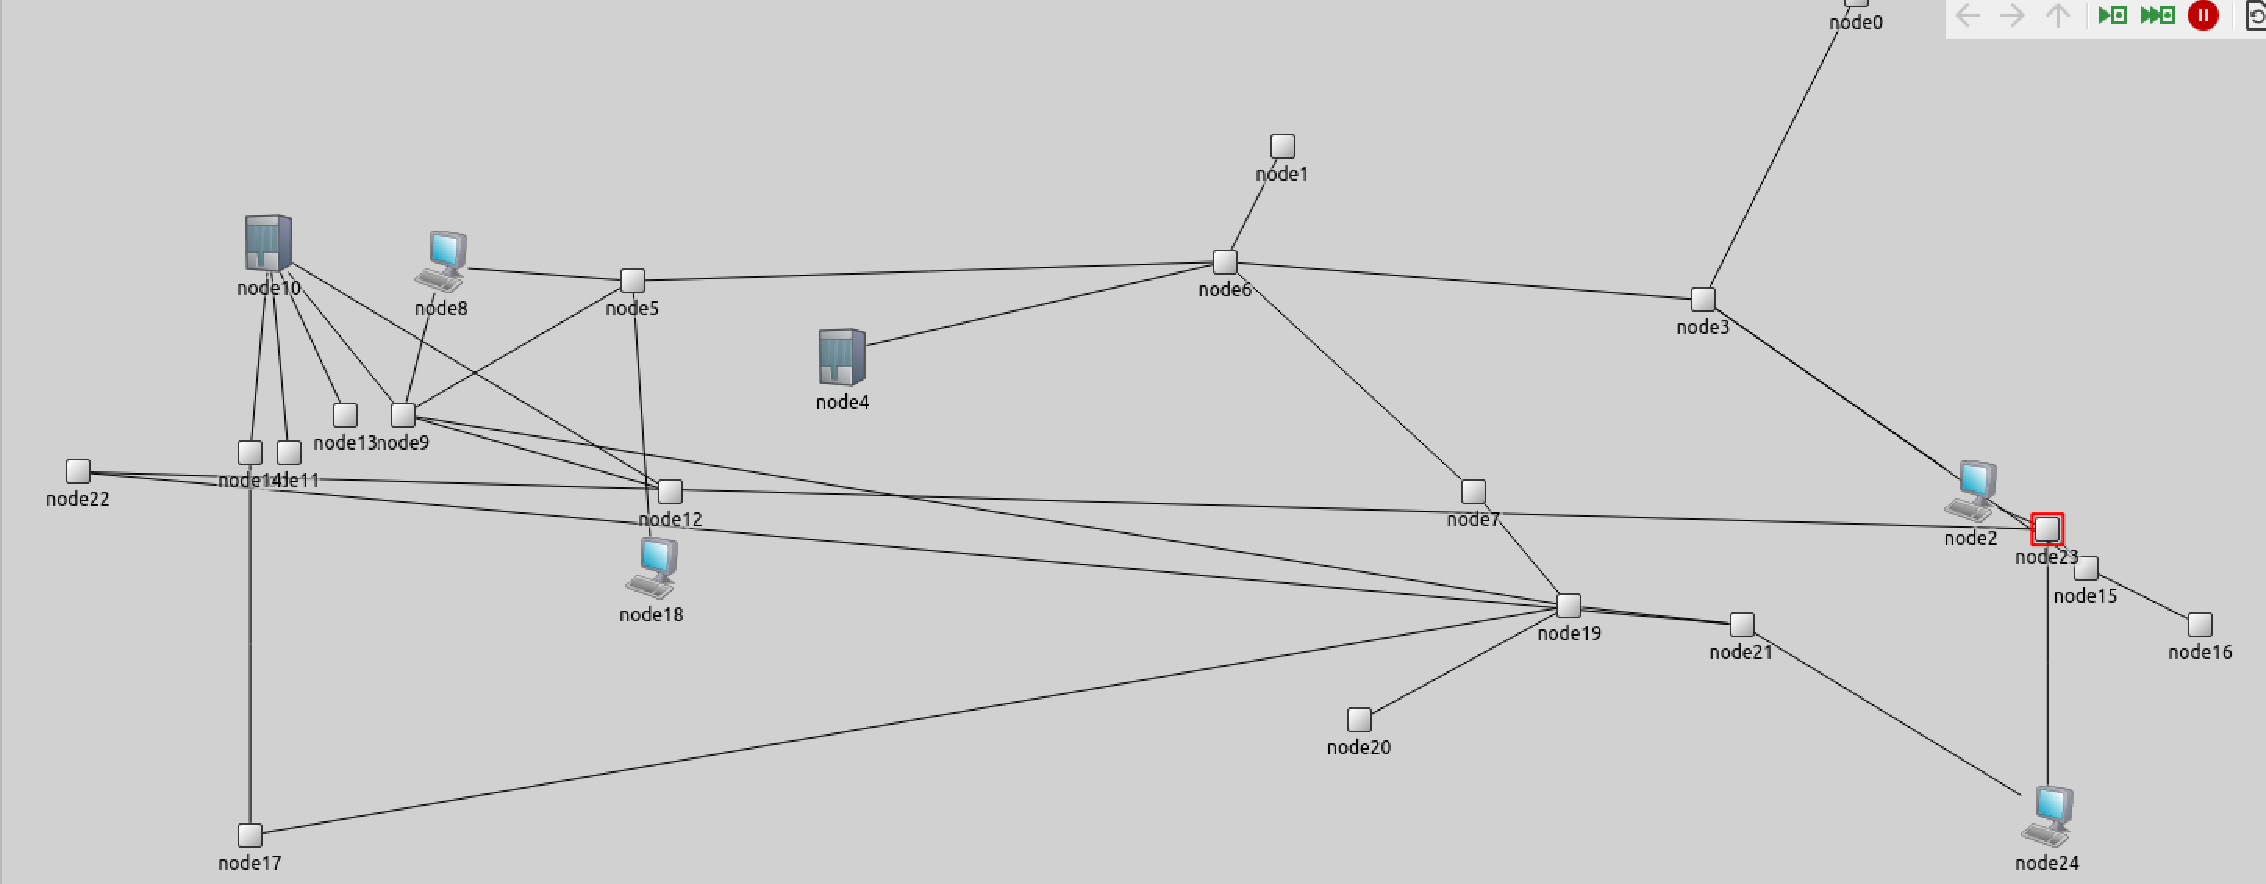
\includegraphics[width=0.5 \textwidth]{figures/MultServerNew}
\caption{This is the multi-server multi-client new topology where the clients are denoted as computers, and the servers are shown as servers. Notably, the topology changed the same way as in fig 5, and new connections that will be used can be seen in red.
}
\end{figure}

\begin{table}[h!]
\centering
\begin{tabular}{|c|c|c|}
\hline
Server Node & Old Topology QPH & New Topology QPH \\ \hline
Server 4 & 333.6 & 340.2  \\ \hline
Server 10 & 331.2 & 327 \\ \hline
\end{tabular}
\caption{Queries per hour at scale factor 0.01 for each server servicing each client under old and new topologies in the multi-server multi-client scenario.}
\label{tab:my_label}
\end{table}

\begin{table}[h!]
\centering
\begin{tabular}{|c|c|c|}
\hline
Server & Old Topology (s) & New Topology (s) \\ \hline
Server 4 & 10.67 & 10.24  \\ \hline
Server 10 & 10.26 & 10.29 \\ \hline
\end{tabular}
\caption{Average time for each server to fulfill the client's queries under old and new topologies in the multi-server multi-client scenario.}
\label{tab:my_label}
\end{table}


\begin{table}[h!]
\centering
\begin{tabular}{|c|c|c|}
\hline
Client/Server Nodes & Old Topology (s) & New Topology (s) \\ \hline
Client 2 Server 4 & 8.01  & 9.82  \\ \hline
Client 8 Server 4 & 8.85  & 9.55  \\ \hline
Client 18 Server 4 & 10.56 & 10.08 \\ \hline
Client 24 Server 4 & 9.03  & 10.23 \\ \hline
Client 2 Server 10 & 10.22 & 10.29 \\ \hline
Client 8 Server 10 & 4.98  & 4.67  \\ \hline
Client 18 Server 10 & 7.61  & 7.73  \\ \hline
Client 24 Server 10 & 10.1  & 10.12 \\ \hline
\end{tabular}
\caption{Average time for each client node to complete its set of queries for each server in the old and new topology in the multi-server multi-client scenario.}
\label{tab:my_label}
\end{table}

In this scenario, two servers can be considered two separate applications running on all clients that each server is trying to service or replicated processes servicing the same clients to increase fault tolerance. Either way, in this scenario, we want to evaluate how changing the topology in a multi-application/multi-server setting can impact the performance metrics of the system(s) as a whole.

For the multi-server multi-client scenario, we consider a 4-client 2-server scenario. The original topology for this scenario builds off the multi-client multi-server original topology by adding a server node randomly assigned a location that turns out to be in the upper left node 10, shown in fig 6. For this topology, we simulated to extract metrics for each server's throughput test and queries per hour test. We first conducted 10 throughput tests, which yielded an average time of 10.67s for server 4 and 10.26s for server 10 to process all of the client's queries, as seen in Table 7.  Also, notably, all the client's completion times for the throughput test are in Table 8. Then we conducted a simulation to record the queries per hour, which, with a scale factor of 0.01 on the database size, yielded queries per hour of 333.6 on server 4 and 331.2 on server 10, as seen in Table 6.

	Having our initial metrics of the system, we can improve the system's performance by performing the same topology changes as the one-server multi-client scenario, as seen in fig 7. Then we use this new topology and extract the same performance metrics again, yielding an average completion time for the throughput tests as 10.24s for server 4 and 10.29s for server 10, as seen in Table 5. Then for queries per hour, server 4 got an average of 340.2, and server 10 got an average of 327, as seen in Table 6.


\subsection{Multi-Server Multi-Client Results and Discussion}

Comparing and contrasting the original and new topologies' performances, we can see that the performance of one server improved while the other did not. Specifically, as seen in Tables 6 and 7, it takes longer for server node 10 to fulfill all client queries during the throughput tests and has fewer queries per hour on the new topology than the original, unlike server node 4, which improves in both categories going from the original to the new topology. Specifically, this is because when transitioning from the old to the new topology, we replaced the connection client node 24 had, which was closer to server node 10, increasing the total latency between client node 24 and server node 10, leading to more delayed communications and delayed services for the client node. Therefore, we observe that changing the topology in a multi-server setting could improve the performance of one server servicing its clients while making it worse for the other servers. 

For client completion times displayed in Table 8, we can see that, like the one server multi-client scenario, the completion times for all clients converged closer to each other for server node 4. In contrast, the server node 10 times stayed relatively the same.  This is because we changed the topology like the one server multi-client scenario. Hence, the convergence of times for the clients in the new topology is because since some of the client nodes' latency decreased due to the topology change, all client nodes have a reasonable chance to be first in line to get query the server. That is why the previously closest nodes increased in completion time in the new topology. Continuing, the client nodes' completion times for server 10 stayed relatively the same since we did not change to change the topology in a way that increased the connectivity between the client nodes and server node 10.

\subsection{Overall Results}

All the scenarios showed that performance benefits could be attained for distributed applications. As for all scenarios, there existed ways of changing the topology to yield better performance.

	The single server single client scenario showed that with a simple tweak in the topology highlighted by Fig 2 and 3, the simple distributed application simulated performance slightly improved, as seen in Tables 1 and 2. This was due to shorter message travel times between the client and server.

	Secondly, the single server multi-client scenario also provided evidence of performance benefits in a slightly more sophisticated setting with more clients. The changes to the topology are highlighted in Fig 4 and 5, and the performance benefits are highlighted in Tables 3 and 4. With this scenario, we saw better performance for the throughput test and queries per hour because we changed the topology.
	
	Lastly, in the multi-server multi-client scenario, the evidence still pointed to the fact that changing the topology could positively impact a distributed application's performance; therefore, its scalability is affected positively as well since its more performant it can handle more users. However, it also showed that in the presence of multiple servers or applications, changing the topology could only benefit one server and even decrease the performance of another. The topologies can be seen in Fig 6 and 7, and the performance statistics in are in Tables 6 and 7. The revelation that other distributed applications could be effected poorly could raise ethical issues on on how to change the topology for every application's benefit.

	Additionally, we saw that the client's throughput test completion times in Tables 5 and 8 were affected by the topology changes too. Specifically, when the topology changed to increase the performance of a server, the completion times of each client converged to be around the same time. This is because it is a single-threaded server, and decreasing the latency between the client nodes' and the server leads to all client nodes having a reasonable chance to be first in line to get query the server. That is why the previously closest nodes increased completion time in the new topology.

	Ultimately, all the scenarios showed that changing the topology can benefit performance.  However, for this study, it only showed minor improvements. 




\section{SUMMARY}

The exponential growth of client-server distributed applications has resulted in the need for scalable and adaptable systems capable of servicing many users. However, the current reliance on static topologies limits the performance and scalability of the applications. 

	Most other works in this area discuss the potential of changing topology and how to change it. However, no evidence or data supports those claims that topology could positively impact preformance. Therefore, our study focused on finding out if there are performance benefits to help scale by changing the topology of applications involved with TPC-H, such as distributed systems involving data warehousing, business intelligence, decision support systems, and online analytical processing.

	For our methodology to solve this problem, we ran simulations in OMNet++ off of an actual topology named AGIS, only assuming a propagation delay. We also assumed we could change the topology of a few main methods today, such as optical switches and SDN. Then we ran simulations for 3 different scenarios a single server single client, single server multi-client, and mult-server multi-client. Each scenario was simulated to extract performance statistics, such as queries per hour and throughput tests for each server.

	Our simulation results indicate that changing the topology can boost performance for applications. However, with the caveat that improving one distributed application's performance can worsen others. These findings pave the way for new developments to manage the topology to leverage the performance benefits dynamically. It also raises ethical issues on if we should change the topology for one application's gain while others stay stagnant or even suffer from the change.



\section{Conclusion}


Overall, our research contribution comes from the increased understanding of the potential performance improvements by changing the topology. It is a stepping stone for future solutions to revolutionize the client-server distributed application. The implications of this study could be the increased use of client-server technology in distributed applications, as businesses may be interested in its increased performance, reliability, and scalability. It could also contribute to the understanding and previously unknown insights into client-server networks.

	Many difficulties in making this study came from a lack of knowledge and inexperience in researching. However, we did learn a lot struggling along the way, so if we were to perform this study again, I would simulate larger scale applications considering transmission delays and traffic in the network. Then by getting the simulations closer to what happens in real-world distributed applications, whatever claims from the data would be more substantial.

Future work could be done to simulate more scenarios in this space and develop topology management solutions to leverage the performance boosts. For example, larger-scale simulations could be done to prove further the claims made in this study, or other groups of applications other than TPC-H could be tested to generalize the claims to more groups of applications. In addition, ethical strides need be made to establish what kind of changes to the topology are morally right so not one application has unfair advantages over another. Once these are done and more evidence is gathered, future work could create dynamic topology managers that change the topology to leverage these performance benefits.






